\documentclass[9pt,twocolumn,twoside]{../../styles/osajnl}
\usepackage{fancyvrb}
\hypersetup{
	colorlinks=true,
	linkcolor=blue,
	filecolor=magenta,      
	urlcolor=blue,
}

\journal{i524} 

\title{Cloudmesh client extension for AWS}

\author[1]{Gregor von Laszewski}
\author[1]{Milind Suryawanshi}
\author[1]{Piyush Rai}

\affil[1]{School of Informatics and Computing, Bloomington, IN 47408, U.S.A.}


\dates{project-006, \today}

\ociscodes{Cloud, I524}

% replace this with your url in github/gitlab
\doi{Report:
	\url{https://github.com/cloudmesh/sp17-i524/blob/master/project/S17-IR-P006/report/report.pdf}\\
	Code: \url{https://github.com/cloudmesh/cloudmesh.aws}}


\begin{abstract}
	
 ASW client is an extension to the Cloudmesh client \cite{www-cloudmesh-client} for ineteracting with Amazon Web Services. Cloudmesh client is command line tool to access numerous cloud envirnments and manage the deployment of virtual machines on them. It has it's own command shell \cite{www-cloudmesh-cmd5}. AWS client extends its capability to work with Amazoz EC2 and is based on Libcloud EC2 driver \cite{www-libcloud-ec2}.
 
\end{abstract}

\setboolean{displaycopyright}{true}

\begin{document}

\maketitle

\section{Introduction}

AWS provides a cloud service to deploy virtual machines (VM) with numerous operating systems environment availble in different flavors. The images are called Amazon Machine Image (AMI) and are available as preconfigured for different applications. Once can also create his own custom environment \cite{www-amazon-ec2}.

The Amazon EC2 drivers provides numerous functionalities to authenticate into the aws, list available configurations and create and boot VMs. The AWS Client is based on cloudmesh.cmd5 and cloudmesh.common. It uses mongodb in the backend to store the cloud information such as list of availble images or instances running on the cloud. Requests library \cite{www-python-requests} is used to connect to the backend through rest services. The rest service is deployed using  cloudmesh REST framework \cite{www-cloudmesh-rest}.

\section{Getting Started}

One needs to create an aws account first to be able to acces its cloud. The instructions for it are available at \cite{www-amazon-aws}. A pair of access key and secret keys are required to be generated to authenticate into the cloud \cite{www-amazon-key}. These keys are required to be kept confidential. These keys are required to be specified in a yaml configuration file. Default vm image and flavor can also be specified in the configuration file. Following are some of the configuration entries:

\begin{verbatim} 
cloudmesh:
  clouds:
    aws:
      credentials:
        EC2_ACCESS_KEY: 'ACCESS KEY'
        EC2_SECRET_KEY: 'SECRET KEY'
        .
        .

    default:
      image: 'IMAGE ID'
      size: 'SIZE ID'
      location: 'LOCATION'
	  
\end{verbatim}

The user need to ensure that the combination of image, size and location is valid and that it's account has the required priviliges for it. The instructions for installation of AWS client can be found at \cite{www-cloudmesh-aws}. Once, the client has been installed and configurations settings enabled, the mongodb and the rest servies to access the database can be started by following command:

\begin{verbatim}
    cms admin mongodb start
    cms admin rest start
\end{verbatim}

The above services will be requried by AWS client to store cloud related information locally. The user can now execute the client commands e.g.:

\begin{verbatim}
    cms aws flavor refresh
\end{verbatim}

This will fetch the list of image sizes available on Amazon EC2 cloud.

\section{Architecture}

The commands are implemented as methods of a class AwsCommand which is based on PluginCommand from cloudmesh shell. Depending on the arguments passed, corresponding routine is called from Aws client API which acts as a wrppaer around the libcloud EC2 drivers and is also responsible to connect with backend database apart from reading the configuratio from yaml file. The entire code is written in Python.

\subsection{Technologies Used}

\begin{enumerate}
	\item Cloudmesh.common and Cloudmesh.cmd5: The common library contains number of modules such as for printing and measuring execution time. The cmd5 is an "dynamically extensible CMD based command shell" [2].

	\item Libcloud EC2 driver: The driver provides a number of functions for various functionalities such as from listing the available nodes to generating a key pair and deplying a VM.

	\item MongoDb: MongoDB is an open source document store database. It's used by AWS client to store information about various VM configuration options available on the Amazon EC2 cloud. It's also used to store information regarding the VMs that are running on the cloud. The information in the database is refreshed whenever it's fetched from the cloud.

	\item Cloudmesh.rest: The cloudmesh rest framework is used to deploy the start the mongodb and rest services. The schema for the objects to be stored in the database is collectively specified in json file called 'all.json'. The schema defined in the file is closely associated with the code in awsclient.py responsible for fetching the information from cloud and passing it to mongodb through rest services. From our expericence during the development of this project, we observed that rest services required the schema to be precise and didn't handle null values for collection fields. There's another file all.settings.py which contains the configuration information for rest services such as port mongodb is running on alongwith the database name. It contains the schema for the collections and the list of methods to be provided by the rest services. The database connectivity was intially developed using pymongo library. However, during the review it was suggested that the code based on pymongo is quite low level and does not have adequate security features. This led to the use of Pyhthon Requests library.
	
\end{enumerate}

\section{AWS Commands}

\begin{enumerate}
	
	\item Refresh: Whether to always fetch the information from the cloud over the network or display it from the local database when asked can be configured by setting the configuration variable 'refresh' to either 'on' or 'off'. When the value is set to on, the onformation will always be fetched from the cloud.
	
	\begin{verbatim}
    cms aws refresh on
	\end{verbatim}
	
	\item Image refresh: The images available on the cloud could be listed using this command. The databse will also be updated with the newly fetched list.
	
	\begin{verbatim}
    cms aws image refresh
	\end{verbatim}
	
	\begin{figure}[h!]
		\centering
		\fbox{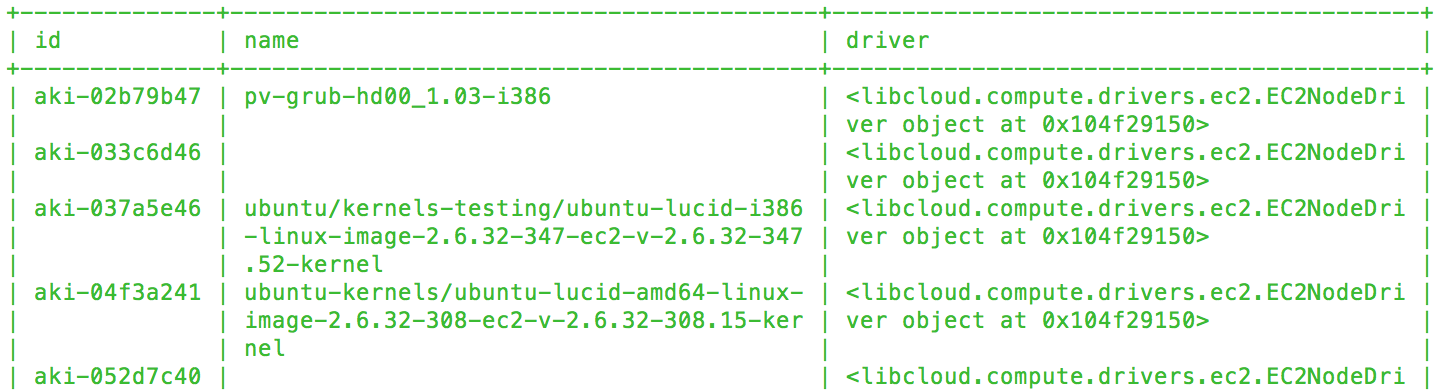
\includegraphics[width=\linewidth]{images/cms_aws_image_refresh.png}}
		\caption{cms aws image refresh}
		\label{fig:imagerefresh}
	\end{figure}
		

	\item Image list: Depending on whether the value of 'refresh' is set to 'on' or 'off', the list is either fetched from the cloud or from the local database.
	
	\begin{verbatim}
    cms aws image list
	\end{verbatim}
	
	\item Flavor refresh: This will list the different sizes of VMs that are available on the cloud. The information is fetched from the cloud and stored locally.
	
	\begin{verbatim}
    cms aws flavor refresh
	\end{verbatim}
		
	\begin{figure}[h!]
		\centering
		\fbox{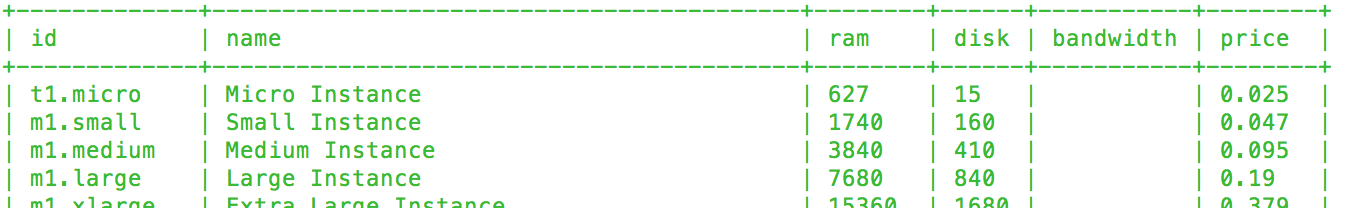
\includegraphics[width=\linewidth]{images/cms_aws_flavor_refresh.png}}
		\caption{aws flavor refresh }
		\label{fig:flavorlist}
	\end{figure}
	
	\item Flavor list: The flavor list is either fetched from the cloud or from the local database depending on whether the value of 'refresh' is set to 'on' or 'off'.
	
	\begin{verbatim}
    cms aws flavor list
	\end{verbatim}
	
    \item Start/Boot vm: Creates a new node instance and start that node automatically. The required parameter is \textit{IMAGE\_ID}. This command assumes user has created keypair with name \textit{AWS1}. The default values; flavor and location being take from cloudmesh.yaml (user need to set those value prior firing the command). You can see the create node instance on console, once it get created.
    
    \begin{verbatim}
    cms aws vm boot IMAGE_ID
    \end{verbatim}
    
   	\begin{figure}[h!]
	   	\centering
	   	\fbox{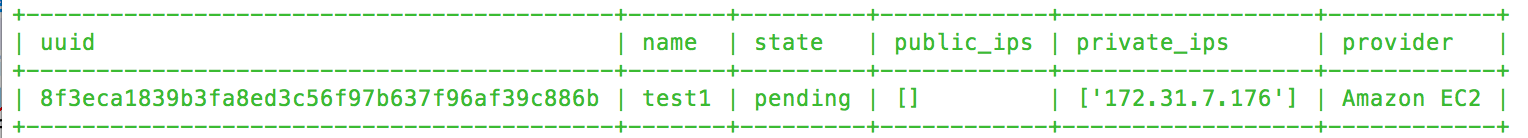
\includegraphics[width=\linewidth]{images/vm_boot_ami-0183d861.png}}
	   	\caption{cms aws vm boot ami-0183d861 }
	   	\label{fig:vmboot}
    \end{figure}

    \item Reboot vm: If vm is running and reboot command fired, running vm gets reboot. The state of the node gets changed from RUNNING to 	REBOOTING. The rebooting time of node depends on the configuration we selected, while creating it. \textit{vm reboot} required \textit{NODE\_UUID}. Once user fired vm list, all the running node \textit{NODE\_UUID} will be shown.
    
    \begin{verbatim}
    cms aws vm reboot NODE_UUID
    \end{verbatim}
    
    \item Delete vm: Destoyes the instance of a node. Also destory all the associated data with that node, including backup. Node will take time to terminate and remove from the list. Once it fired, very first the state of the node changes to \textit{TERMINATED} and after certain time it will get remove from node list as well. 
    
    \begin{verbatim}
    cms aws vm delete UUID
    \end{verbatim}
    
    \item List created vm : List out all the created nodes present in different states for aws.
    
    \begin{verbatim}
    cms aws vm list
    \end{verbatim}
    
     \begin{figure}[h!]
    	\centering
    	\fbox{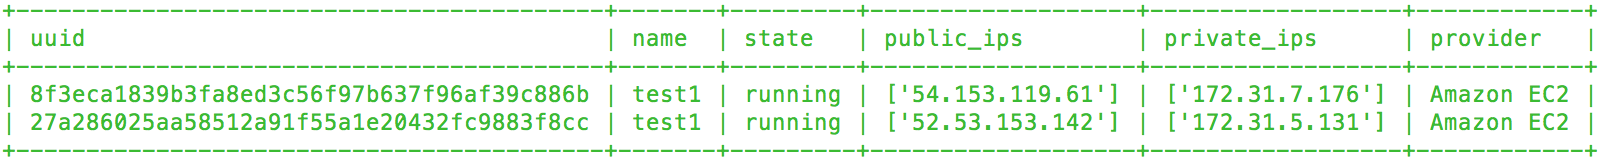
\includegraphics[width=\linewidth]{images/vm_list.png}}
    	\caption{cms aws vm list }
    	\label{fig:vmlist}
    \end{figure}

    \item Create keypair: To create the node, one of the essential component is \textit{key pair}. Amazon EC2 uses public key to encrypt and decrypt the password and then recipient uses private key to decrypt it. This public and private keys are know as a \textit{key pair}. User needs to give any (alpha numeric) name to that key.
    
    \begin{verbatim}
    cms aws keypair create NAME
    \end{verbatim}
    
    \begin{figure}[h!]
    	\centering
    	\fbox{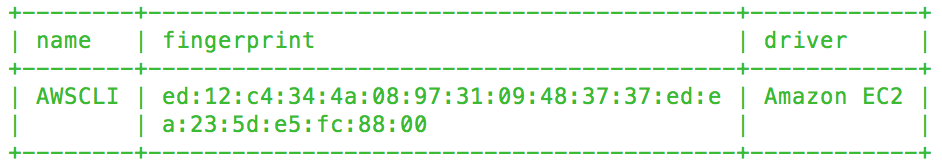
\includegraphics[width=\linewidth]{images/cms_aws_keypair_create.png}}
    	\caption{cms aws keypair create AWSCLI}
    	\label{fig:keypaircreate}
    \end{figure}

    \item Delete keypair: Allows user to delete created \textit{key pair}, which is no longer in use.
    
    \begin{verbatim}
    cms aws keypair delete NAME
    \end{verbatim}
    
    \item List created keypairs: List out all the created \textit{key pairs}.
    
    \begin{verbatim}
    cms aws keypair list
    \end{verbatim}
    
    \item Get keypair: Returns the key pair object, which has the name of \textit{key pairs}, driver and hash key.
    
    \begin{verbatim}
    cms aws keypair get NAME
    \end{verbatim}
    
    
    \item Get locations: It will show all the available locations associated with Amazon EC2 account. For free tier, user will get two locations. More locations will be available in paid service.
    
    \begin{verbatim}
    cms aws location list
    \end{verbatim}
    
    \begin{figure}[h!]
    	\centering
    	\fbox{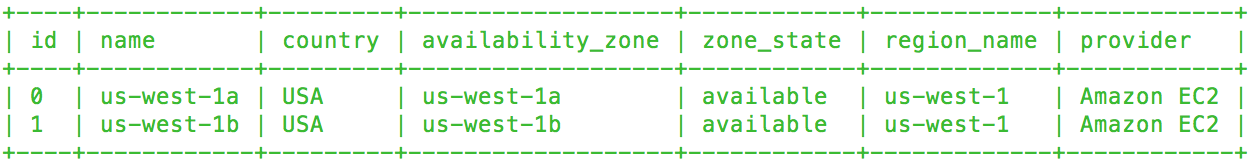
\includegraphics[width=\linewidth]{images/cms_aws_location_list.png}}
    	\caption{cms aws location list}
    	\label{fig:locationlist}
    \end{figure}

    \item Create volume: Creates the volume for vm, the size of volume is in GB, the default value is set to 1 GB. The maximum number of volumes that we can attach to vm will be depends on its operating system.
    
    \begin{verbatim}
    cms aws volume create VOLUME_NAME
    \end{verbatim}
    
    \begin{figure}[h!]
    	\centering
    	\fbox{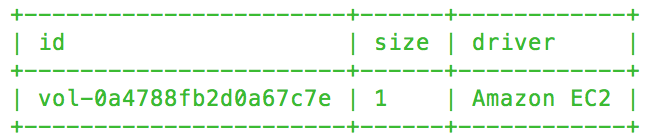
\includegraphics[width=\linewidth]{images/cms_aws_volume_create_VOL_TEST_1.png}}
    	\caption{cms aws volume create VOL\_TEST\_1}
    	\label{fig:createvolume}
    \end{figure}
     
    \item List created volumes: Command shows the created volumes with the id, size and the driver name.
    
    \begin{verbatim}
    cms aws volume list
    \end{verbatim}
    
    \begin{figure}[h!]
    	\centering
    	\fbox{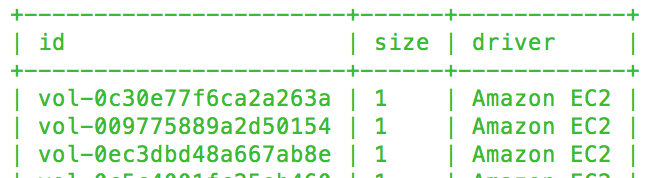
\includegraphics[width=\linewidth]{images/cms_aws_volume_list.png}}
    	\caption{cms aws volume list}
    	\label{fig:volumelist}
    \end{figure}
    
    \item Delete volume: User can delete the unwanted volumes using the \textit{VOLUME\_ID}.
    
    \begin{verbatim}
    cms aws volume delete VOLUME_ID
    \end{verbatim}
    
    
\section{Create AWS Node}
	To create own node instance, following steps need to be followed. 

\subsection{Prerequisite}

\begin{enumerate}
	\item User should have a valid AWS account.
	\item \href{https://console.aws.amazon.com/iam/home?#/users}{Create a IAM}  user for which the access and secret key being generated. After creating user, access key and secret key gets generated, copy that keys \cite{www-attach-policy}.
	\item Once the user has created, now add permission to created user
		\begin{enumerate}
			
			\item visit \href{https://console.aws.amazon.com/iam/home} {IAM home}
			\item select \textbf{policie}s in left hand menu
			\item create \textbf{administrator policy} from amazons existing policies
			\item select \textbf{administrator checkbox} and \textbf{attach} to your user
		\end{enumerate}
	\item Open the ../cloudmesh.yaml configuration file and update with EC2\_ACCESS\_KEY, EC2\_SECRET\_KEY, you just copied. Now set default flavor, image and location, as t2.micro, ami-0183d861 and us-west-1 respectively in same file.
	\item Mongodb server should be up and running (please refer section 2. Getting started)

\subsection{Create Node}

\begin{enumerate}
	\item Create keypair name using command
	
	\begin{verbatim}
	cms aws keypair create  AWS1
	\end{verbatim}
	
	It will create the \textit{keypair name}, it is essential to create the \textit{node}. To verify it, \textit{cms aws keypair list} command will list down all created \textit{keypairs} so far.
	
	\item Now create the node 
	
	\begin{verbatim}
	cms aws vm boot ami-0183d861
	\end{verbatim}
	
	Above command will create a node instance with the image of ami-0183d8661.

\end{enumerate}	
	
\end{enumerate}


\subsection{Create Node}

\end{enumerate}

\section*{Acknowledgements}

Prof. Gregor von Laszewski originally suggested this project and provided the objectives in simplistic form. He reviewd the code as it was developed during the course of this project. His inputs helped us to make the code more secure and efficient. He provided us with different resources to look for help and overcome the challenges faced during the course.

% Bibliography

\bibliography{references}
 
\section*{Author Biographies}
\begingroup
\setlength\intextsep{0pt}
\begin{minipage}{1.0\columnwidth}
  \noindent
  {\bfseries Milind Suryawanshi} received his BE (Electronics and Telecommunication) in 2010 from
  The University of Pune. His research interests include Big Data analytics for intelligence and research. 
\end{minipage}
\begin{minipage}{1.0\columnwidth} 
  \noindent
  {\bfseries Piyush Rai} received his BE (Computer) in 2011 from
  The University of Pune. His research interests also include Big Data analytics for military intelligence and frinancial markets. 
\end{minipage}

\endgroup

\newpage

\appendix

\section{Work Breakdown}

The work on this project was distributed as follows between the
authors:

\begin{description}

\item[Milind Suryawanshi.] Explored the libcloud EC2 drivers, investigated the various arguments requried by their different routines and implemented their use accordingly.

\item[Piyush Rai.] Worked on configurable parameters and database connectivity using pymongo and rest services.

\end{description}


\end{document}
